\documentclass[11pt,a4paper]{article}
\usepackage[utf8]{inputenc}
\usepackage[T1]{fontenc}
\usepackage{lmodern}
\usepackage[margin=2.5cm]{geometry}
\usepackage{booktabs}
\usepackage{graphicx}
\usepackage{caption}
\usepackage{float}
\usepackage{amsmath}
\usepackage{breqn}
\usepackage[hidelinks]{hyperref}

\title{An automatic report for the dataset: sales: units}
\author{Some Math empowered by some AI guided by some researchers}
\date{09 November 2026}

\begin{document}
\maketitle

\noindent\emph{Produced by \texttt{autostat}, a Python 3 port of the Automatic Bayesian Covariance Discovery system of Lloyd et al. (AAAI 2014).}


\begin{figure}[H]
\centering
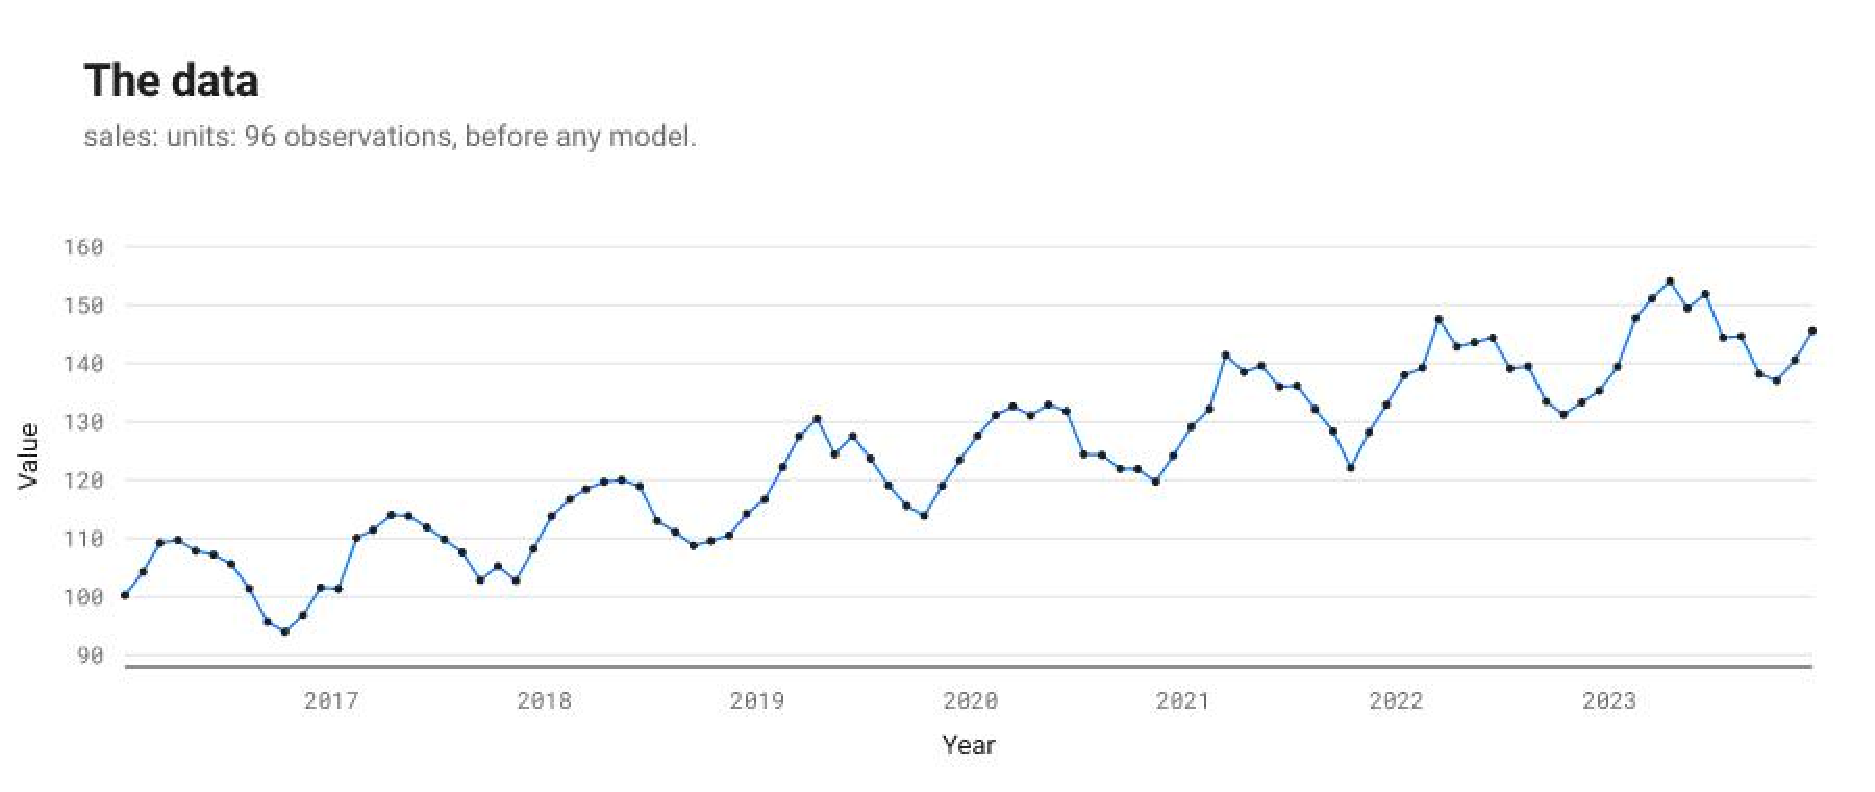
\includegraphics[width=\linewidth]{data.pdf}
\caption*{The data}
\end{figure}

\section*{Executive summary}

The structure search selected \texttt{Lin + WN + Per} (Bayesian information criterion 449.2; negative log likelihood 210.9 on 96 points). It decomposes into 3 additive components, listed by how much each reduces extrapolation error:
\begin{enumerate}
  \item A linearly increasing function.
  \item A periodic function with a period of 1.0 years.
  \item Uncorrelated noise.
\end{enumerate}

\begin{center}
\begin{tabular}{lrrrr}
\toprule
\# & $R^2$ cumulative (\%) & Residual variance explained (\%) & CV MAE & MAE reduction (\%) \\
\midrule
data & & & 124 & \\
1 & 83.8 & 83.8 & 5.16 & 95.8 \\
2 & 98.4 & 90.3 & 1.58 & 69.3 \\
3 & 100.0 & 100.0 & 1.58 & -0.0 \\
\bottomrule
\end{tabular}
\end{center}

MAE: mean absolute error over ten contiguous held-out blocks; CV: cross-validated.

\section*{The formula found}

The structure search is a symbolic regression: it searches a grammar of expressions over kernels and keeps the one with the lowest Bayesian information criterion. This is the expression it kept, with every fitted parameter in place; $t$ is in years.
\begin{dmath*}
y(t) = f_{1}(t) + f_{2}(t) + f_{3}(t)
\end{dmath*}

Each component is a Gaussian process with its own covariance:
\begin{dmath*}
f_{1}(t) \sim \mathrm{GP}\!\left(0,\ 37.14\,(t - 2000)(t' - 2000)\right)
\end{dmath*}
\begin{dmath*}
f_{2}(t) \sim \mathrm{GP}\!\left(0,\ 31.71\,\frac{\exp\!\left(0.01596\cos\frac{2\pi (t - t')}{1}\right) - I_0(0.01596)}{e^{0.01596} - I_0(0.01596)}\right)
\end{dmath*}
\begin{dmath*}
f_{3}(t) \sim \mathrm{GP}\!\left(0,\ 3.578\,\delta_{t t'}\right)
\end{dmath*}

These components have a closed form, read from their posterior mean:
\begin{dmath*}
f_{1}(t) = 99.63 + 6.095\,(t - 2016)
\end{dmath*}
\begin{dmath*}
f_{2}(t) \approx 7.95\cos\!\left(\frac{2\pi \cdot (t - 2016)}{1} - 1.807\right) + 0.3961\cos\!\left(\frac{2\pi \cdot 2 \cdot (t - 2016)}{1} - 0.9546\right)
\end{dmath*}

A periodic kernel is exactly a sum of cosines, so a periodic component is a Fourier series in its period; it is written up to the harmonic after which the rest weighs less than 0.1 % of the component, hence the approximate sign.

The other components are smooth, quasi-periodic or noise without a short formula: a draw from such a process has no finite closed form; its covariance above is the formula.

Closed form of each component:

\begin{center}\footnotesize
\begin{tabular}{lp{0.36\linewidth}l}
\toprule
\# & component & closed form \\
\midrule
1 & A linearly increasing function & exact polynomial of degree 1 \\
2 & A periodic function with a period of 1.0 years & Fourier series, 2 harmonics, largest gap 0.027 \% of the component \\
3 & Uncorrelated noise & none: the covariance is the formula \\
\bottomrule
\end{tabular}
\end{center}

\section*{Search path and stopping criterion}

The 2014 configuration searches a fixed number of levels and keeps the lowest BIC; it has no stopping rule. The table follows the winner of each level. A change of structure adds or removes terms; a level that keeps the structure only refits its parameters. BIC differences read on the scale of Kass and Raftery (1995): under 2 barely worth mentioning, 2 to 6 positive, 6 to 10 strong, over 10 very strong.

\begin{center}\footnotesize
\begin{tabular}{lllp{0.36\linewidth}lll}
\toprule
level & BIC & change & structure & components & closed & params \\
\midrule
1 & 569.4 &  & WN + SE & 2 & 0 & 3 \\
2 & 464.8 & -104.6 & WN + Per x SE + SE & 3 & 0 & 7 \\
3 & 458.4 & -6.4 & WN + Lin x SE + Per x SE & 3 & 0 & 8 \\
4 & 453.8 & -4.6 & Lin + WN + Per x SE & 3 & 1 & 7 \\
5 & 449.2 & -4.6 & Lin + WN + Per & 3 & 2 & 6 \\
6 & 449.2 & -0.0 & Lin + WN + Per & 3 & 2 & 6 \\
7 (kept) & 449.2 & -0.0 & Lin + WN + Per & 3 & 2 & 6 \\
\bottomrule
\end{tabular}
\end{center}

\begin{figure}[H]
\centering
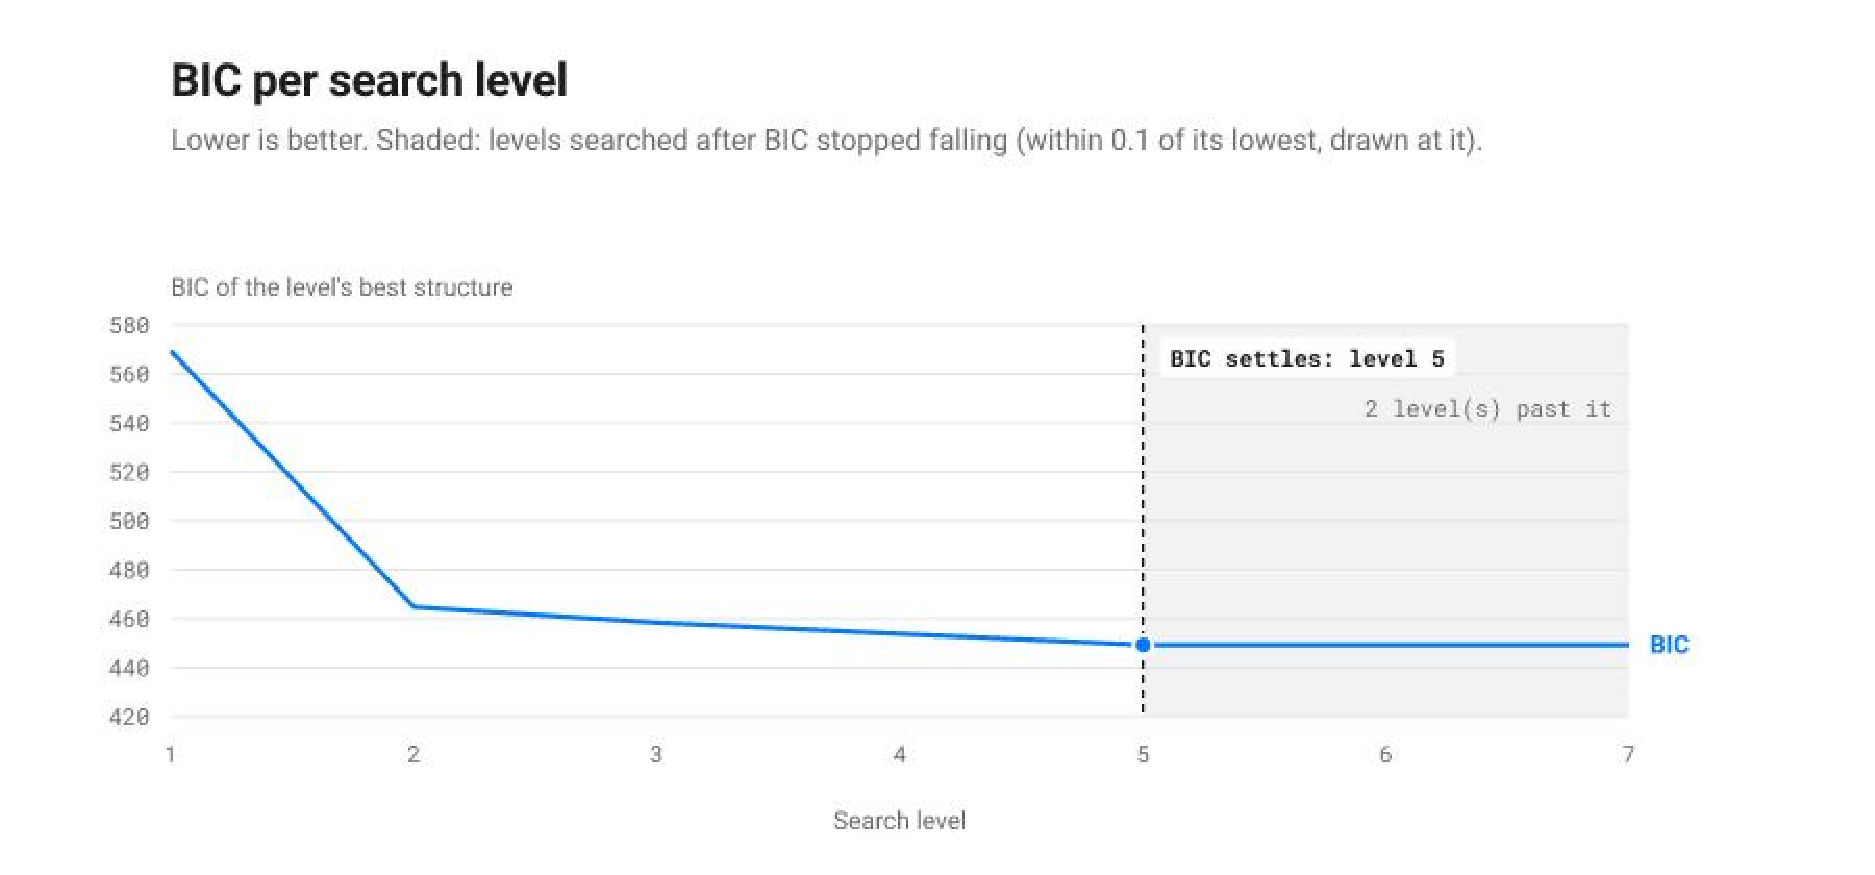
\includegraphics[width=\linewidth]{bic.pdf}
\caption*{BIC per search level}
\end{figure}

Posterior weight of each structure met, exp(-BIC/2) normalised under a flat prior, after the Bayesian machine scientist (Guimerà et al., 2020): where the search keeps one structure, the weights say how much the data prefer it to the others. The 2 structure(s) under 0.001 are left out.

\begin{center}\footnotesize
\begin{tabular}{p{0.36\linewidth}ll}
\toprule
structure & lowest BIC & weight \\
\midrule
Lin + WN + Per & 449.2 & 0.899 \\
Lin + WN + Per x SE & 453.8 & 0.092 \\
WN + Lin x SE + Per x SE & 458.4 & 0.009 \\
\bottomrule
\end{tabular}
\end{center}

\begin{itemize}
\item The search ran 7 levels (stopping after 2 level(s) without a BIC fall above 0.1, at most 20) and keeps the model of level 7, Lin + WN + Per, BIC 449.2.
\item That structure was first reached at level 5; the levels after it only refitted its parameters, lowering BIC by 0.0 in all.
\item The best different structure, Lin + WN + Per x SE (level 4), is 4.6 above it: positive evidence for the kept one on the Kass and Raftery scale.
\item Weighed by exp(-BIC/2) under a flat prior, as the Bayesian machine scientist weighs expressions, the structures met give the kept one a posterior weight of 0.899 and the next, Lin + WN + Per x SE, 0.092: the data favour the kept one without ruling the next out.
\item BIC stopped falling at level 5. The 2 level(s) searched past it kept its structure and lowered BIC by 0.00 in all, less than the tolerance of 0.1: going on buys nothing the data pay for.
\item A rule stopping after 1 level(s) without a fall above 0.1 would have ended the search at level 6 and kept the same structure, less refitted.
\item A rule stopping after 2 level(s) without a fall above 0.1 would have ended the search at level 7 and kept the same model.
\item The kept expression has 6 parameters for 96 points: its BIC is a fit term 2 NLL = 421.9 plus a complexity term p ln n = 27.4, each extra parameter costing 4.56; it splits into 3 components, 2 of them with a closed form.
\end{itemize}

\begin{figure}[H]
\centering
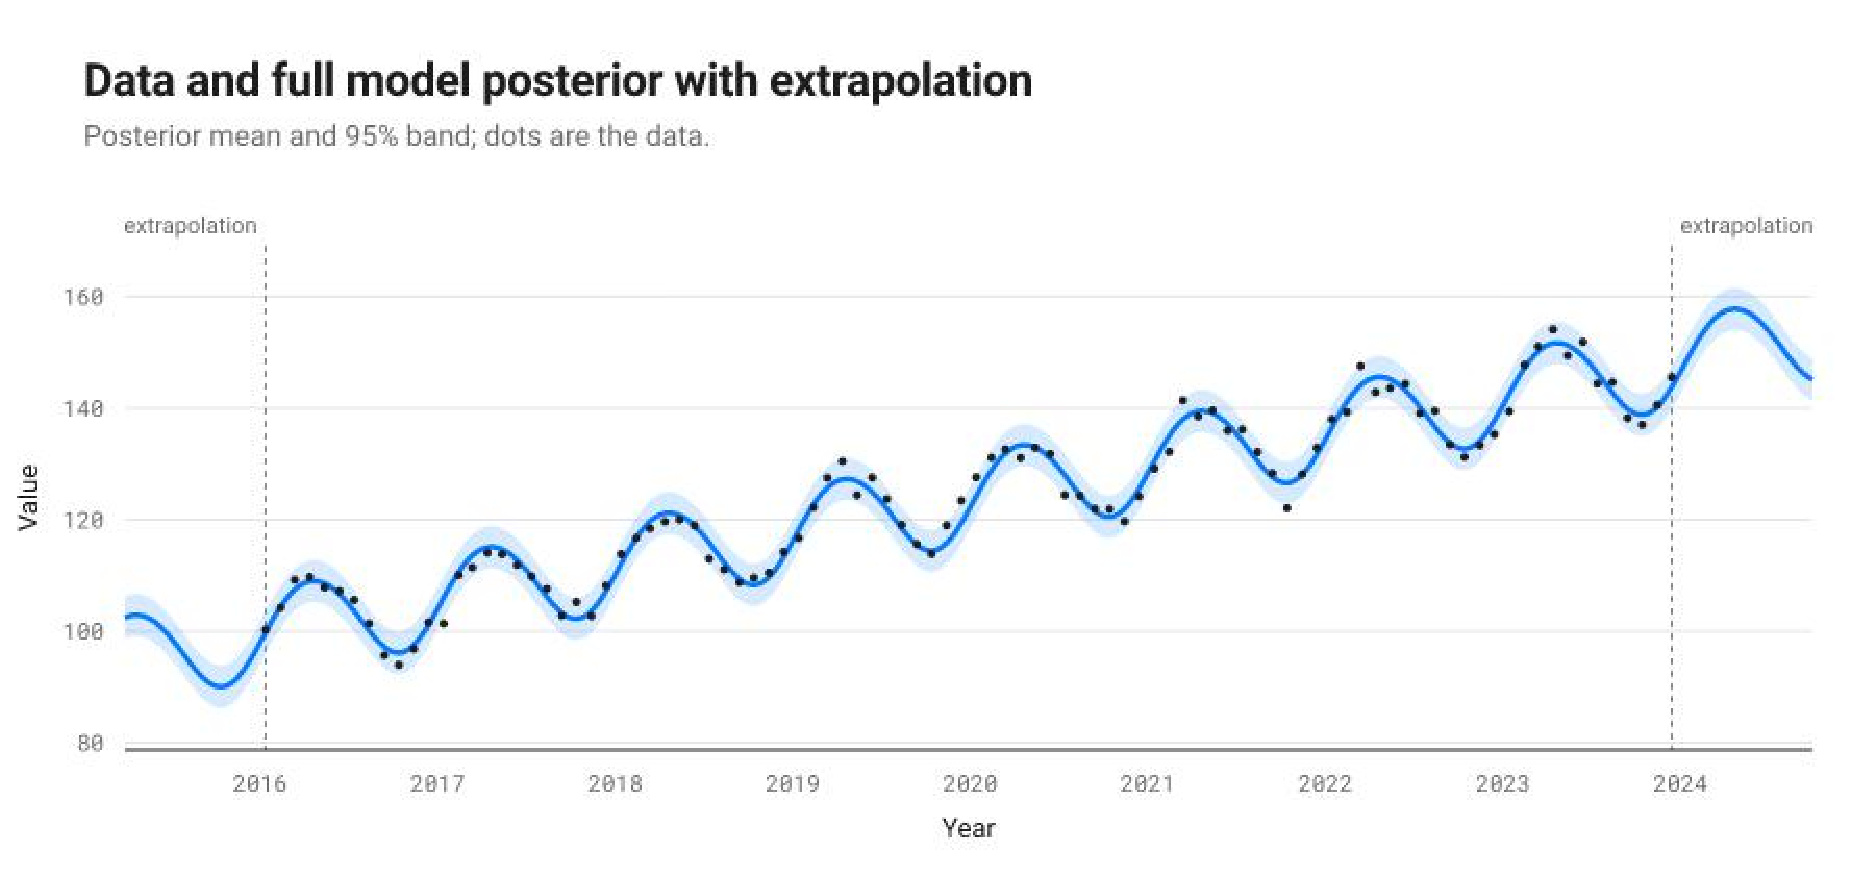
\includegraphics[width=\linewidth]{fit.pdf}
\caption*{Data and full posterior}
\end{figure}

\section*{Detailed discussion of the components}

\subsection*{Component 1: A linearly increasing function}

This component is linearly increasing.

This component explains 83.8\% of the data's variance on its own; with the components above it, 83.8\%. Adding it changes the cross-validated MAE by -95.8\%.

\emph{Extrapolation.} This component is assumed to continue to increase linearly.

\begin{figure}[H]
\centering
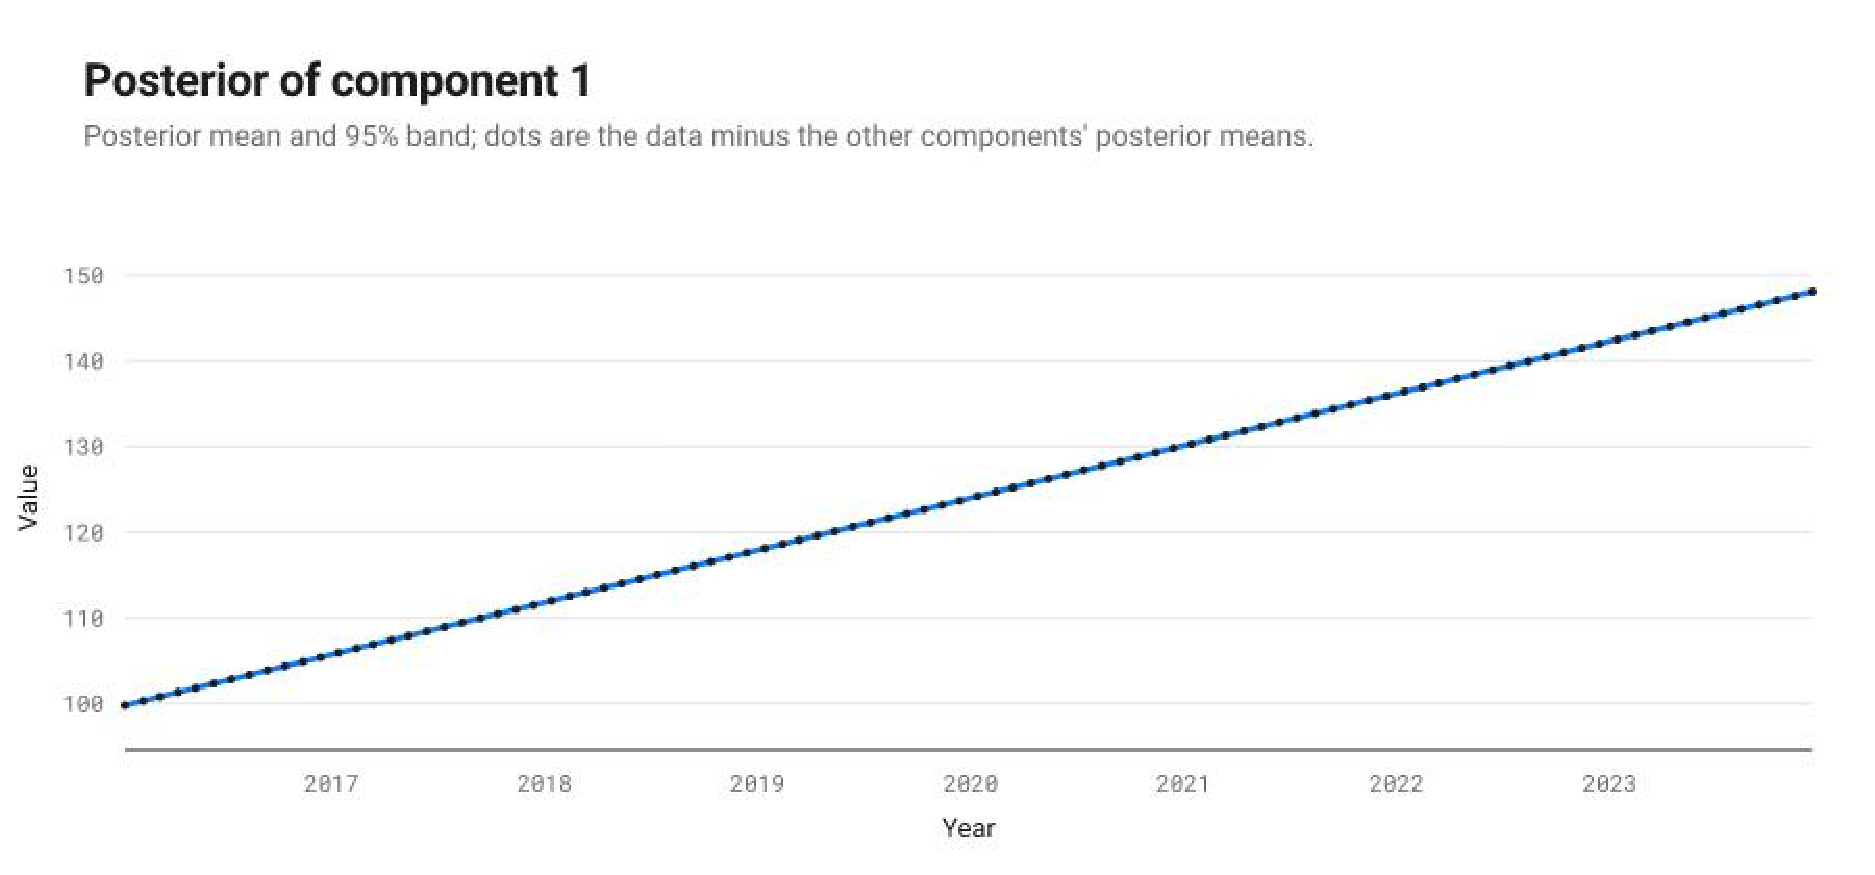
\includegraphics[width=\linewidth]{component_1.pdf}
\caption*{Component 1}
\end{figure}
\subsection*{Component 2: A periodic function with a period of 1.0 years}

This component is periodic with a period of 1.0 years. The shape of this function within each period is very smooth and resembles a sinusoid.

This component explains 7.7\% of the data's variance on its own; with the components above it, 98.4\%. Adding it changes the cross-validated MAE by -69.3\%.

\emph{Extrapolation.} This component is assumed to continue periodically with a period of 1.0 years.

\begin{figure}[H]
\centering
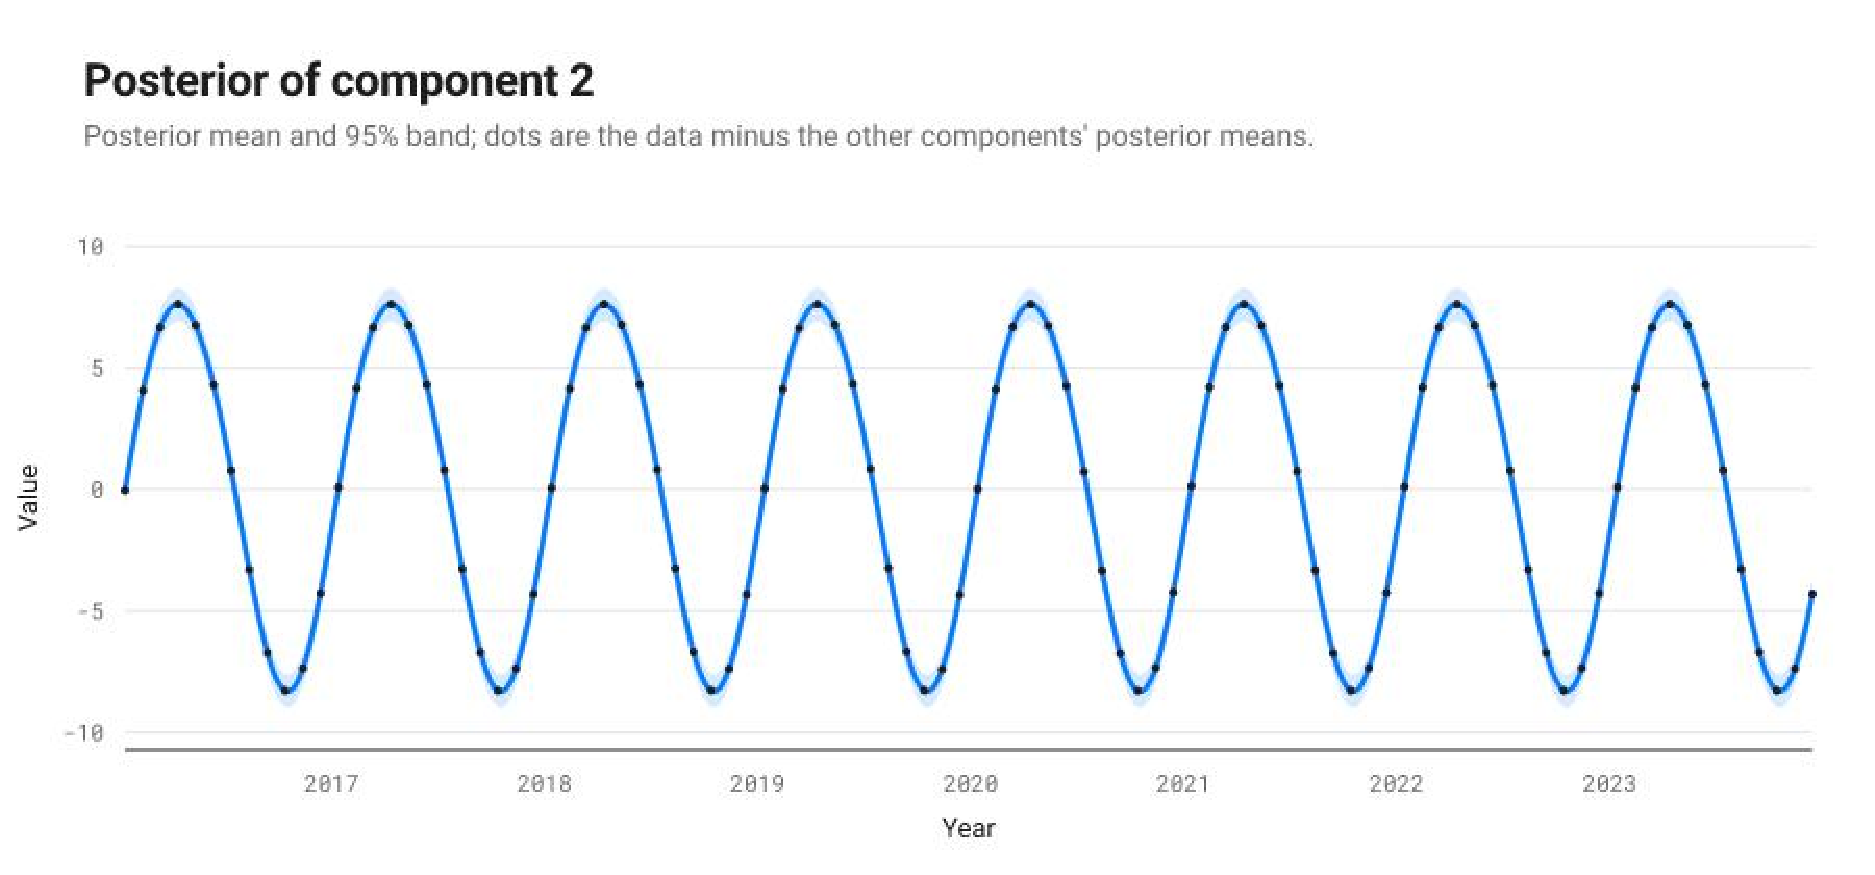
\includegraphics[width=\linewidth]{component_2.pdf}
\caption*{Component 2}
\end{figure}
\subsection*{Component 3: Uncorrelated noise}

This component models uncorrelated noise.

This component explains 1.7\% of the data's variance on its own; with the components above it, 100.0\%. Adding it changes the cross-validated MAE by 0.0\%.

\emph{Extrapolation.} This component assumes the uncorrelated noise will continue indefinitely.

\begin{figure}[H]
\centering
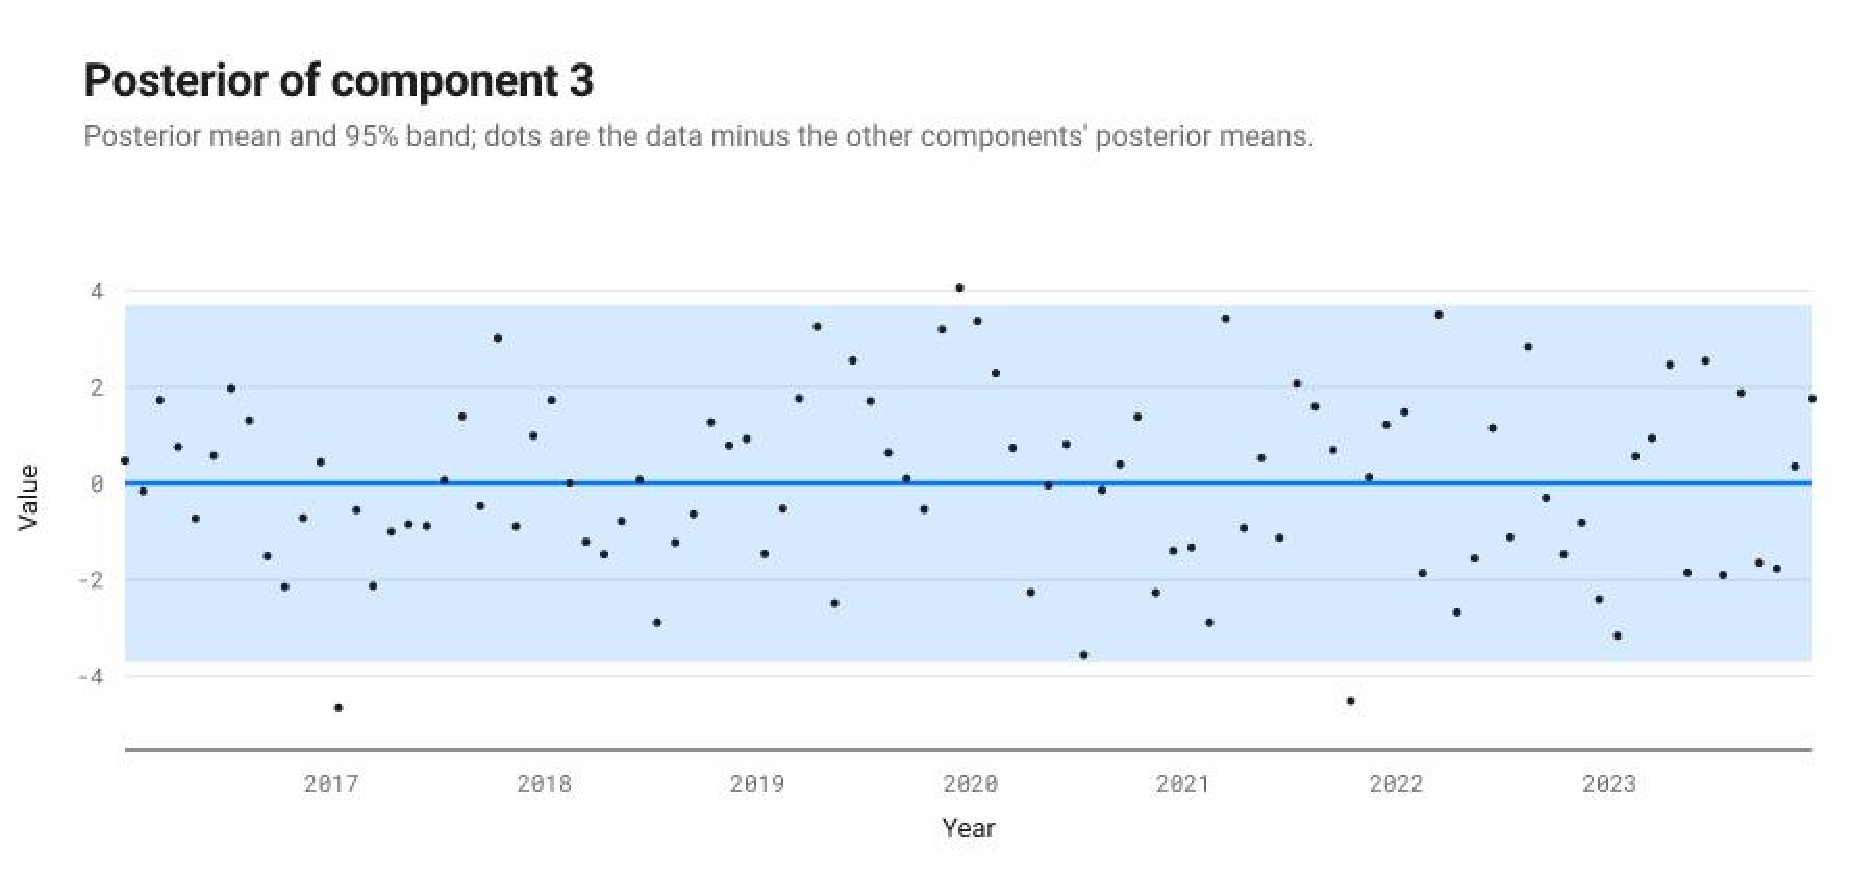
\includegraphics[width=\linewidth]{component_3.pdf}
\caption*{Component 3}
\end{figure}

\section*{Model checking}

Not computed for this report (\texttt{describe(..., check=False)}).

\end{document}
